\documentclass[a4paper,10pt,oneside,openany]{jsbook}
\renewcommand{\figurename}{Fig.}
\renewcommand{\tablename}{Table.}
\bibliographystyle{junsrt}  % 電子情報通信学会の論文誌スタイルになってる
\usepackage{amsmath,amssymb}
\usepackage{bm}
\usepackage{cite}
% \usepackage{epsbox}  %図表貼りつけ関連.epsファイルを扱う

\usepackage[dvipdfmx]{color}
\usepackage[dvipdfmx]{graphicx}
\usepackage{verbatim}
\usepackage{wrapfig}
\usepackage{ascmac}
\usepackage{makeidx}
\usepackage{here}
\usepackage{subfigure}
%subcaption ON
%\usepackage[hang,small,bf]{caption}
%\usepackage[subrefformat=parens]{subcaption}
%\captionsetup{compatibility=false}
%tableに色つけ
\usepackage{colortbl}
%図とかの位置 H
\usepackage{here}
%\usepackage{subfigure}

% セクション、サブセクションの文字の大きさ
\makeatletter
\def\@makechapterhead#1{
\vspace*{2\Cvs}
{\parindent \z@ \raggedright \normalfont
\Huge\headfont
\ifnum \c@secnumdepth >\m@ne
\if@mainmatter
\@chapapp\thechapter\@chappos
\hskip1zw
\fi
\fi
#1\par\nobreak
\vskip 3\Cvs}}
\makeatother
%hogehoge 
\makeindex
% 余白・文字数調整(左30mm, 右20mm, 上下共30mm, 文字数約40字/行, 行数約32行)
\setlength{\textwidth}{160truemm}      % テキスト幅: 210-(30+20)=160mm
\setlength{\fullwidth}{\textwidth}     % ページ全体の幅
\setlength{\oddsidemargin}{30truemm}   % 左余白P
\addtolength{\oddsidemargin}{-1truein} % 左位置デフォルトから-1inch
\setlength{\topmargin}{30truemm}       % 上余白
\setlength{\textheight}{237truemm}     % テキスト高さ: 297-(30+30)=237mm
\addtolength{\topmargin}{-1truein}     % 上位置デフォルトから-1inch
\makeatother
\begin{document}
% タイトル設定
%\thispagestyle{empty}
\begin{center}
	{\Huge 手指使用量の常時計測のためのウェアラブルデバイスの開発}\\
	\vspace{2mm}
	{\Large A wearable device for continuous monitoring of fingers activity}\\
	\vspace{7mm}
	{\Huge 松本 崇斗}\\
	\vspace{2mm}
	{\Large Takato MATSUMOTO}\\
	\vspace{10mm}
	{\Large (2017年度入学, 17646137)}\\
	\vspace{25mm}

	\begin{figure}[H]
		\begin{center}
			\vspace{7mm}
			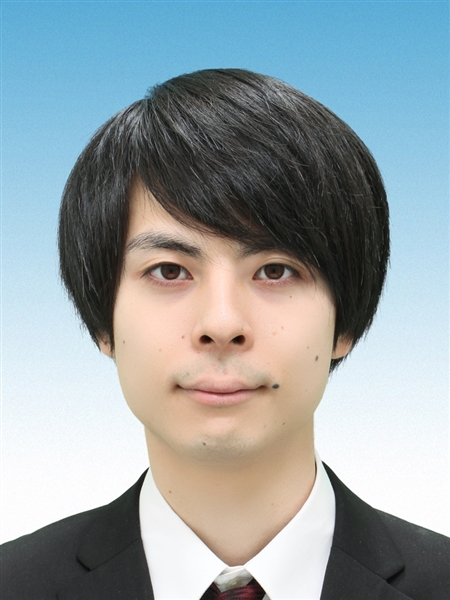
\includegraphics[width=45mm]{face_photo.jpg}
		\end{center}
	\end{figure}

	\vspace{25mm}
	{\Huge 指導教員 近藤敏之 教授}\\
	\vspace{12mm}
	{\Large 東京農工大学 工学府 情報工学専攻}\\
	\vspace{2mm}
	{\Large 2018年度修士論文}\\
	\vspace{2mm}
	{\Large (2018年1月30日 提出)}\\
\end{center}
\frontmatter
% 論文要旨
\thispagestyle{empty}
\begin{center}
	{\large 東京農工大学 工学府 情報工学専攻 2018年度 修士論文 要旨}\\
	\vspace{8mm}
	{\Large 題目 手指使用量の常時計測のためのウェアラブルデバイスの開発}\\
	\vspace{2mm}
	{\large A wearable device for continuous monitoring of fingers activity}\\
	\vspace{8mm}
	{\large 学籍番号 17646137  氏名 松本 崇斗 (Takato MATSUMOTO)}\\
	\vspace{2mm}
	{\large 提出日 2018年1月30日}\\
	\vspace{4mm}
\end{center}














% 目次
\tableofcontents

\mainmatter

%!TEX root = _thesis.tex
\chapter{序論}

\section{はじめに}
脳卒中麻痺リハビリテーションの目標は,食事,更衣,入浴などの日常生活動作ができるように患者の麻痺肢機能を改善することである.麻痺肢機能の改善を促進する介入方法の有効性を評価するためには,介入後の日常生活において,患者の麻痺肢使用量が実際に増えたか否かについて,リハビリテーションの効果を定量的に測る手法が必要である.しかしながら,病院やリハビリ施設で実施する検査では,質問紙やヒアリングによる調査が主体であり,日常生活における麻痺肢使用量を正確に評価することができない\cite{Taub2006,Rand2009}.さらに,診療所や研究所で行われるテストでは,日常生活上での患者の麻痺肢使用量を計測することができない.現在,日常生活上の麻痺肢使用量を測定する手法として,Accelerometryが一般的である.しかし,この手法は加速度センサを用いており,手指の使用量を正確に計測,評価することができない.そのため,本研究では日常生活において,麻痺患者の麻痺肢使用,特に,手指の使用量を計測,評価する手法を提案する.

\section{日常生活動作(Activities of Daily Living)}
日常生活動作(ADL)とは食事,更衣,入浴など,日常生活を営む上で不可欠な基本的な動作のことである.上肢麻痺患者の多くは,日常生活動作をするのに必要な,肢機能が健常者に比べ低い\cite{Zeiler2017}.ADLの向上には,上肢機能の回復が不可欠である.

セラピストは患者の回復度合いや,上肢機能によって,リハビリテーションの手法や計画を決める.
eviudence-based clinical practice

\section{上肢機能評価結果を用いた臨床判断}
麻痺肢機能評価から導かれた結果は,臨床医が患者の麻痺肢機能を治療,回復させる計画を立てる際に,非常に重要である\cite{Lang2013}.加えて,臨床医が麻痺障害後の麻痺肢機能や,その障害の回復を予測する際,麻痺肢機能評価の結果を用いて判断を行う.複数の疫学的なデータから麻痺の回復は,時間経過と関係があると示唆されており,最も障害の回復が見込める期間は
,障害が引き起こってから三カ月以内であると言われている.麻痺の早期の障害の度合いは,最終的な運動障害に関係しており,軽度の障害である場合は,短期間で障害が回復し,3$\sim$6週間前後で障害が完治する可能性が高い\cite{Langhorne2011}.



\section{診療所や研究所で行われる上肢機能の評価手法}
\subsection*{Action Research Arm Test}
Action Research Arm Test\cite{Hsieh2009,Lang2008,Lang2013,Lang2017,Nijland2010,VanDerPas2011,VanDerLee2004,Taub1998}は片側不全麻痺の患者の上肢機能評価手法である
.この手法は19項目を握る,把持,ピンチ,全身運動の四つのサブスケールに
分け評価する手法である.上肢機能は各項目ごと0から3の四段階で評価され,各項目の評価が3であり,合計評価が57である場合,健常者と同等の上肢機能であると評価される.
\begin{figure}[H]
\begin{center}
\begin{tabular}{cc}
\subfigure[ARAT Kit]{
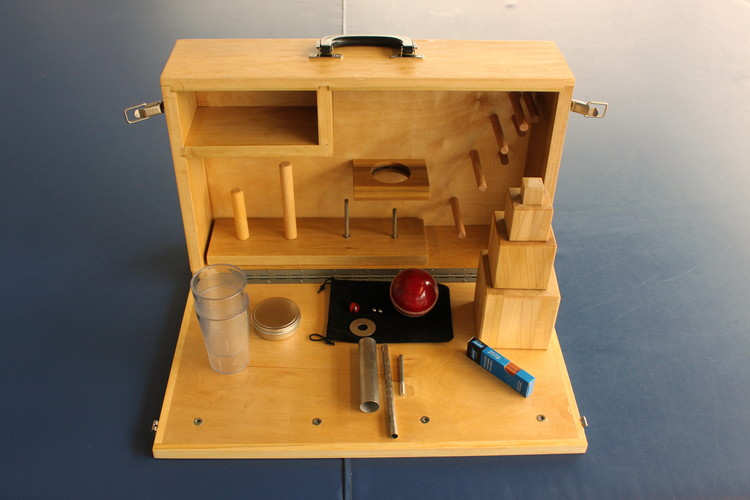
\includegraphics[scale=0.3]{fig/ch1/ARAT_kit}
} &
\subfigure[ARAT Score Sheet]{
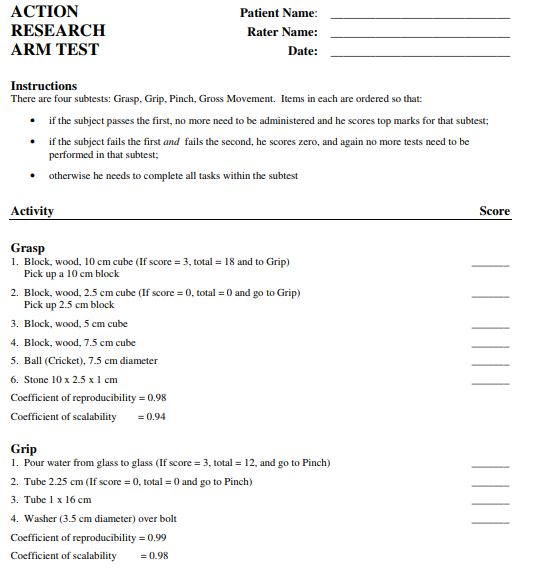
\includegraphics[scale=0.3]{fig/ch1/ARAT_SCORING}
} \\
\end{tabular}
\end{center}
   \caption{Action Research Arm Test\cite{Hsieh2009}}
\label{fig:ARAT}
\end{figure}


\subsection*{Box and Block Test}
Box and Block Test\cite{T.2005,Mathiowetz1985,Desrosiers1993,Lin2010}は実施が簡単かつ実施時間が短い上肢機能評価手法であり,ブロックの把持,移動,解放動作を評価する手法である.
被験者は,1分間で多くのブロックを箱から別の箱に移動させることを指示される.この手法では,上肢機能の能力を1分間に動かしたブロックの個数で評価する.
\begin{figure}[H]
  \centering
  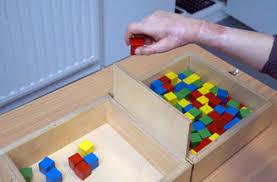
\includegraphics[width=0.8\linewidth]{fig/ch1/babt}
  \caption{Block and Block Test\cite{T.2005}}
  \label{fig:babt}
\end{figure}

\subsection*{Chedoke Arm and Hand Activity Inventory}
Chedoke Arm and Hand Activity Inventory\cite{Barreca2004,Barreca2006,Barreca2005,Johnson2017}は腕,手の麻痺障害後の回復度合いを評価する指標である.
両手の使用を必要とするタスク13項目により,評価を行う.項目ごとに1$\sim$7の7段階で評価され,1は7の25\%以下の腕,手のパフォーマンスを意味する.
よって,高いスコアは,高い,腕や手のパフォーマンスを示す.タスクを行う時間が患者への負担となる場合,この手法を短時間で実施する手法として,Chedoke Arm and Hand Activity Inventory-9,Chedoke Arm and Hand Activity Inventory-8やChedoke Arm and Hand Activity Inventory-7といった手法がある.

\subsection*{Nine-Hole Peg Test}
Nine-Hole Peg Test\cite{Mathiowetz1985,Croarkin2004,Sunderland1989}
は手の器用さを測る簡単な手法である.被験者はペグをホールに刺し,刺した九つのペグを全て抜き取ることを指示される.テストの開始からペグを全て取り終えるまでの時間を計測し,その時間により,被験者の手の器用さを評価する.
\begin{figure}[H]
  \centering
  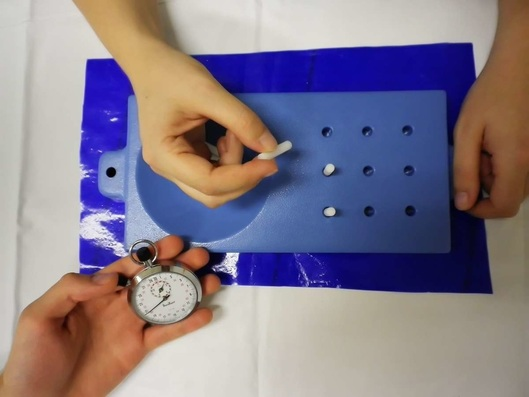
\includegraphics[width=0.8\linewidth]{fig/ch1/nhpt}{}
  \caption{Nine-Hole Peg Test}
  \label{fig:nhpt}
\end{figure}

\subsection*{Wolf Motor Function Test}
Wolf Motor Function Test\cite{Lin2010,Hsieh2009,Shima2009,Nijland2010}
は15個のタスクを含む上肢機能と患者の活動度合いを評価する手法である.1$\sim$6のタスクは関節の動きについて,7$\sim$15のタスクは総合的な上肢機能の評価項目である.患者は時間内にタスクをどれだけ遂行できたか(Functional Ability Score)で評価され,0はタスクを全く完了できないことを意味し,5はタスクを完全に完了できたことを意味する.時間での評価では,短い時間でタスクを完了できた場合,高い上肢機能であると評価する.
\\
上記の手法は,患者の運動機能を計測,評価することが可能である.しかし,これらの手法は日常生活上での患者の麻痺肢使用量を計測することができない.

\section{セルフレポート評価手法}
\subsection*{Motor Activity Log}
片上肢麻痺患者の日常生活上での麻痺肢使用量を測る標準的手法としてMotor Activity Log(MAL)\cite{Taub2006,Uswatte2005,Uswatte2000,Winstein2003,Michielsen2012}がある.MALは,医師が患者に対し,麻痺肢使用の量と質について直接問う,質問形式の手法である.MALの質問項目は,一般的な日常生活動作に関する質問である.日常生活動作とは,電気のスイッチをオンにする動作や引き出しを開ける動作といった,日常生活を営む上で最低限必要な動作である.MALの評価用紙をFig.\ref{fig:Motor Activity Log}に示す.MALの質問項目は30項目あり,日常生活動作時の麻痺肢使用の量と質について11段階の評価で患者が答える.研究所や診療所で行われるリハビリテーションテストは正確に患者の日常生活上での上肢機能を測定できない問題があるが,MALは上記の問題を解決できる上肢機能測定評価の標準的な手法の一つである.

\begin{figure}[H]
\begin{center}
\subfigure[Score sheet]{
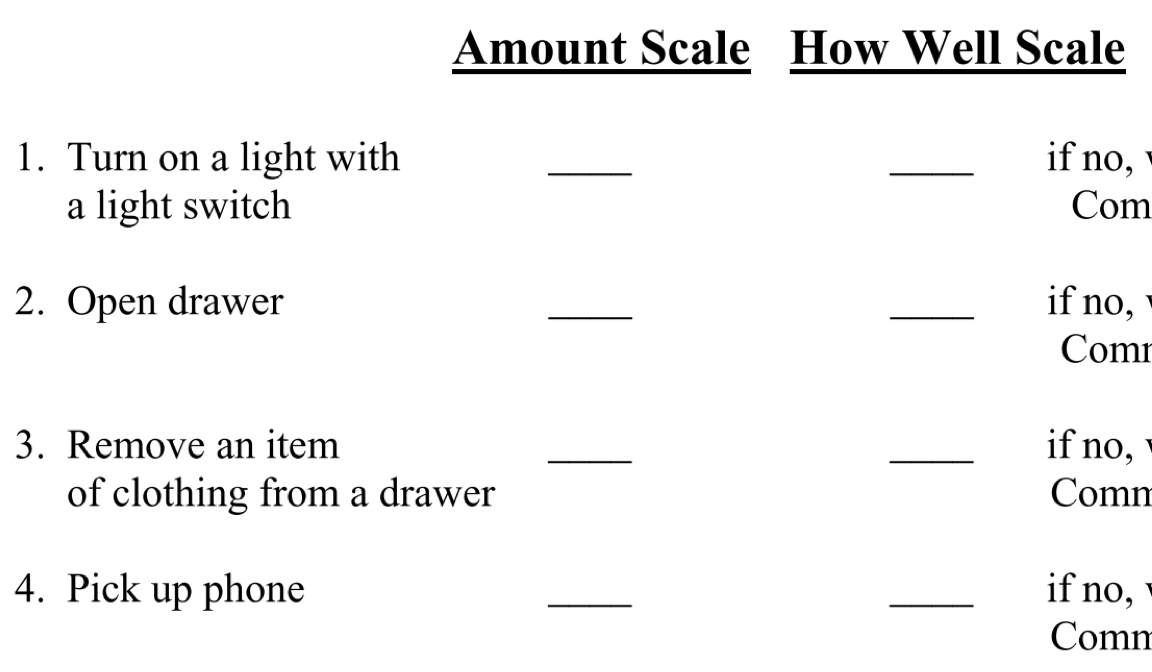
\includegraphics[scale=0.5]{fig/ch1/mal}
}
\begin{tabular}{cc}
\subfigure[Amout Scale]{
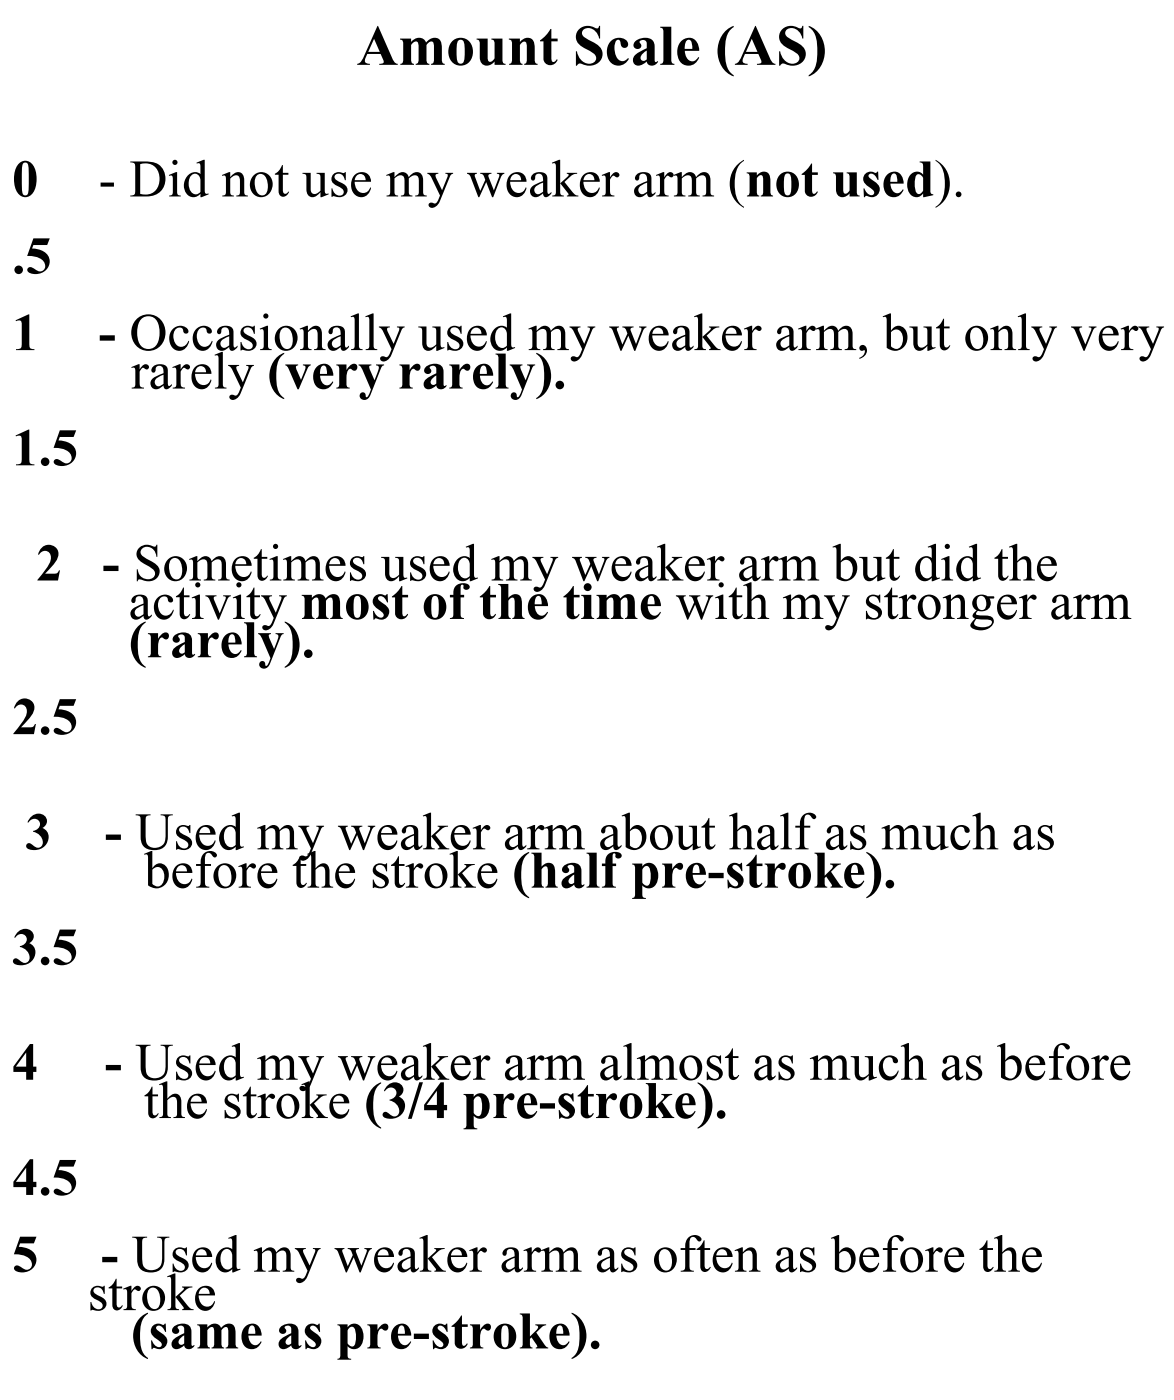
\includegraphics[scale=0.3]{fig/ch1/amount}
} &
\subfigure[How Well Scale]{
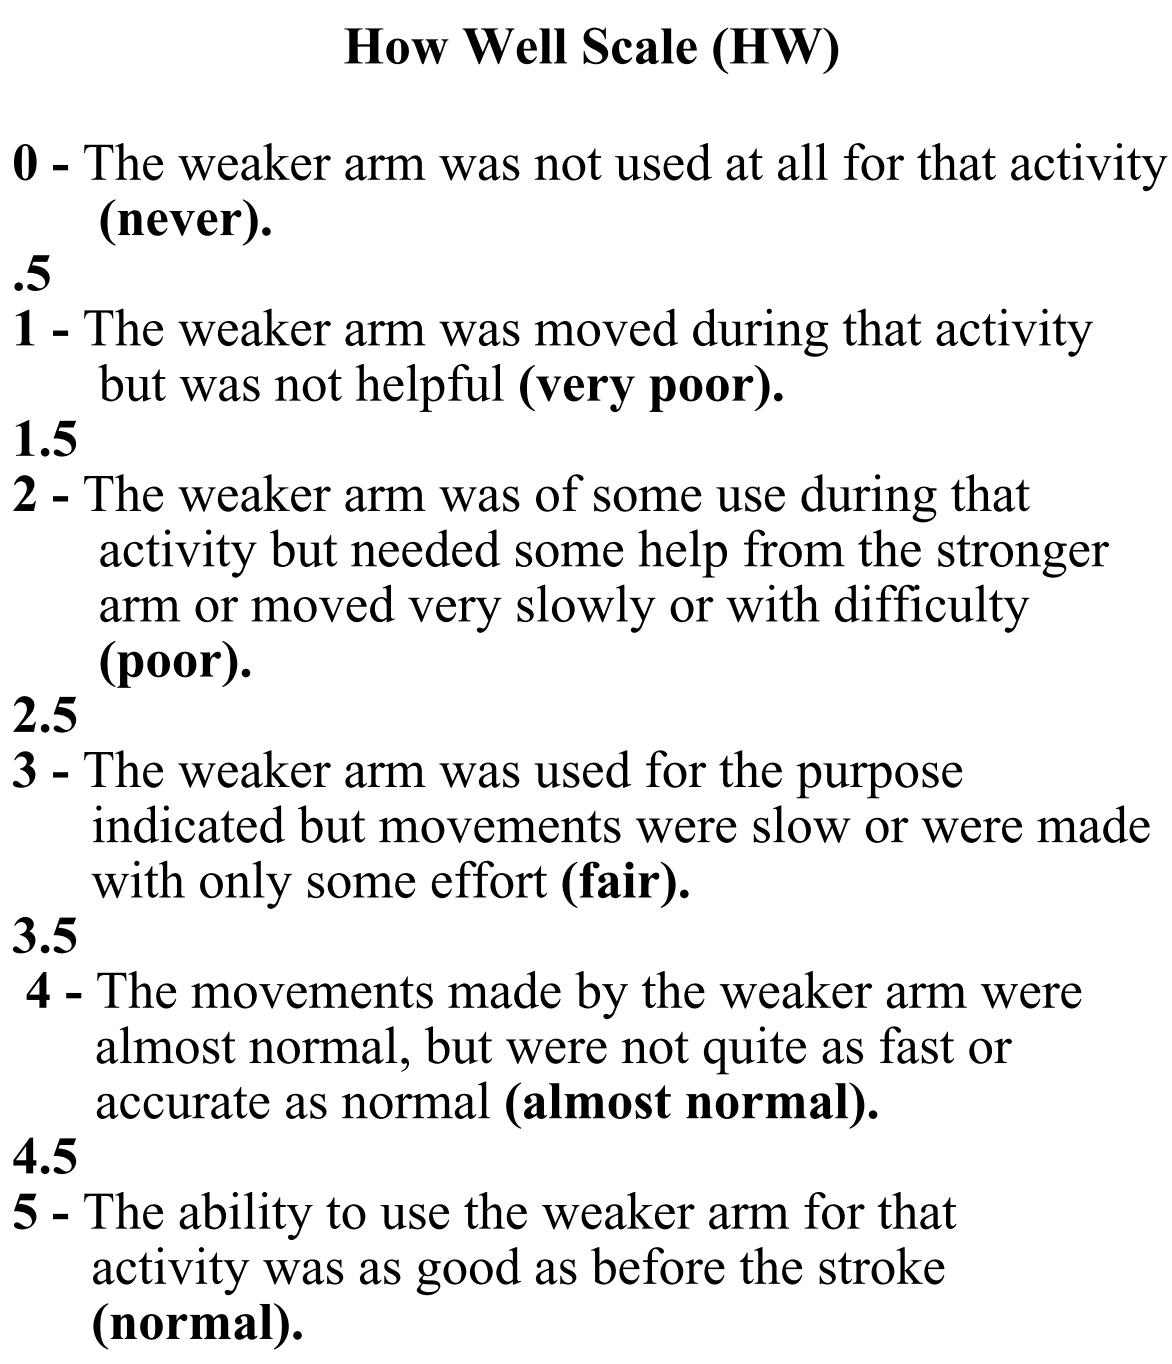
\includegraphics[scale=0.3]{fig/ch1/how}
} \\
\end{tabular}
\end{center}
   \caption{Motor Activity Log\cite{Taub2006}}
\label{fig:Motor Activity Log}
\end{figure}

MALは,質問形式といった測定結果が患者の認知レベルによる影響や質問者の主観的影響を受ける問題がある.例えばHow wellスケールの質問では,患者に対しあるタスクをどれほど良くできたかを問う.タスクを良くできたか悪くできたかは,患者の主観によって左右される.さらにAmountスケールの質問では,患者に対しあるタスクをどれほど多く,麻痺肢を使い行なったかを問う.この質問に答えるためにはタスク行なったかどうかを認知しておく必要がある.加えてMALは質問の回答に患者の記憶が依存するため,患者がタスクを行なったことを忘れてしまう問題がある他,患者に日常生活上でどんなタスクを行なったかを覚えておくよう指示しなければならず,患者に負担がかかる問題がある.これらの理由から,客観的かつ患者に負担がかかりにくい日常生活上での上肢機能測定手法が必要である.

\subsection*{Stroke Impact Scale}
Stroke Impact Scale(SIS)\cite{Lin2010b,Lin2010a,Lai2002,Duncan2001,Duncan2002,Duncan2002a,Duncan2003}は脳卒中のセルフレポート評価手法である.SISの評価項目は,強度,手の機能,ADL,IADL,モビリティ,コミュニケーション,感情,記憶と思考,
そして参加/役割機能の8つの分野に分かれている.患者は自身で5点のリッカート尺度を使用して各項目の能力を評価する.
手の機能とADL,IADLのサブスケールは,上肢機能の測定に最も関連性があるとされている.
各サブスケールのスコアは0から100の範囲であり,健常者のセルフレポートスコアは各サブスケールにおいて100で示される.
SISの実施は対面式のインタビュー形式,電話,または郵便により行われる.郵便で行われた大規模なSISは被験者への負担が大きく,脳卒中の被験者の50\%が自分でアンケートを完成させることができなかった.

\if0
\begin{table}[H]
  \centering  
  \caption{Performance and self-report measures commonly used to assess upper extremity function after stroke\cite{Lang2013}}
  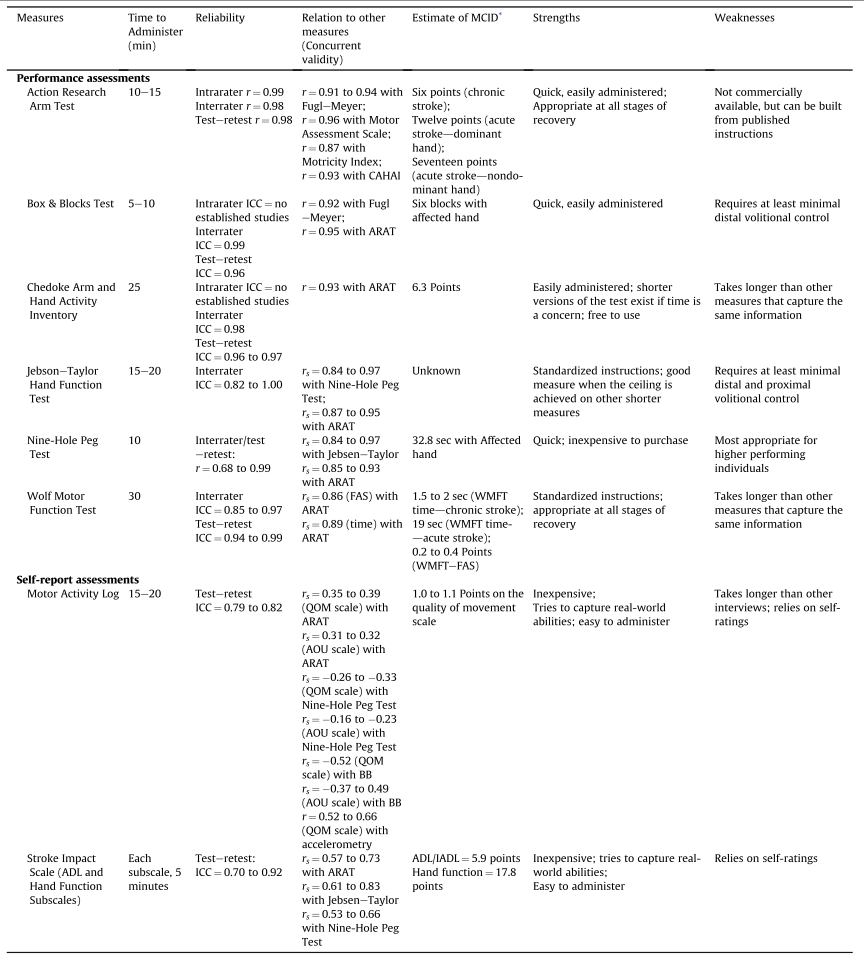
\includegraphics[width=1.0\linewidth]{fig/table1}
  \label{table:measure}
\end{table}
\fi

\section{定量的上肢使用量計測に関する研究}
\subsection*{Accelerometry}
Accelerometry\cite{Chen2005,Hayward2016,Dwiputra2017,VanDerPas2011,VanDerLee2004,Thrane2011,Seitz2011}をFig.\ref{fig:Accelerometry}に示す.Accelerometryは腕の使用量が多ければ,大きな加速度が記録され,腕の使用量が少なければ,記録される加速度は小さいといったことを
仮定したシンプルな腕の使用量の評価手法である.
日常生活動作とともに発生する,腕の加速度を記録する.

Accelerometryは,加速度計が埋め込まれた腕時計型のウェアラブルデバイスで上肢の使用量を測る手法である.Accelerometryは麻痺肢の手首に装着することで,麻痺肢の使用量を測定する.データ記録装置とバッテリーが内蔵されているため,麻痺肢使用量の常時計測に向いている\cite{VanDerPas2011}.しかし,この手法で計測される加速度データはノイズを多く含み,信頼性の高いデータを得ることができない.加速度データに混入するノイズは,測定された加速度が所定の時間内に,閾値を超える場合にのみ,麻痺肢使用のスコアを増加するといった手法の閾値フィルタを用いて低減することができる.このアプローチによって得られたスコアは日常生活において,腕を動かした時間と高い相関を持つことが示されている.しかし,閾値フィルタを使用したノイズ低減を行った場合,加速度が閾値に達しない小さな手の動きが見落とされる可能性がある.また,加速度計が手首に装着されているため,手指の精密な動きを計測できない問題がある.これらの理由から,Accelerometryは指の使用量の測定には向かない\cite{Uswatte2000}.
また,Accelerometryはタスクを行なっているのか,歩行時に手を振っているのかということを見分けられない.歩行時に腕を振っていることを検知する手法があるが,この手法は,足やつま先などに追加のAccelerometryを装着することを必要とする\cite{Ullery2015}.
さらに,Accelerometryはどのタスクをしているのかを見分けることも難しい\cite{Hayward2016}.
\begin{figure}[H]
  \centering
  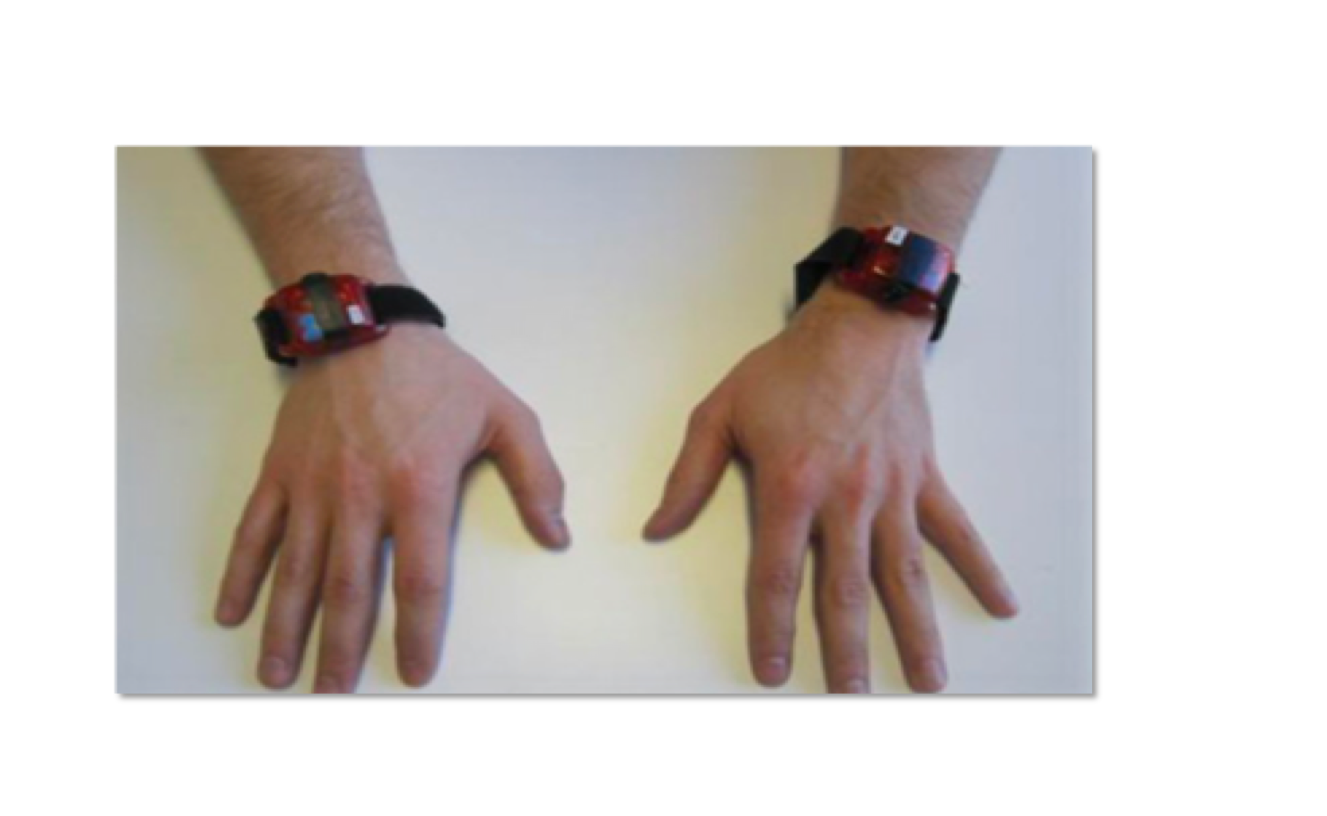
\includegraphics[width=0.8\linewidth]{fig/ch1/acc}
  \caption{Accelerometry\cite{Chen2005}}
  \label{fig:Accelerometry}
\end{figure}

Accelerometryの信頼性と妥当性
Accelerometryが有効であるためには,信頼性と妥当性が高くなければならない.\cite{}同じAccelerometryを使用している場合,ユーザが行なっているタスクが同じであるなら,Accelerometryの加速度の合計値は,同じでなければならない.また,異なるAccelerometryを使用している場合でも,ユーザ間の信頼性が確立されている場合,加速度の合計値は同じタスクに対し一致しなければならない.
Accelerometryは脳卒中患者と健常者の上肢使用量の違いを区別することができる.さらに,accelerometryはリハビリ介入後の上肢使用量の増加,減少を示すことができる.Accelerometryによる上肢機能の評価は,診療所や研究所で行われる上肢機能の評価と高い相関を持っている.

\begin{table}[H]
  \caption{Relationships Between Accelerometer Metrics and Measures of Function According to the ICF}
  \label{table:measure}
  \centering
  \begin{tabular}{ll}
    \hline
    Measure & Correlation\\
    \hline \hline
    Action Research Arm Test &$r = 0.40–0.59$\cite{Lang2007,Rand2012}\\
    Wolf Motor Function Test &$r = 0.62$\cite{Lang2007}\\
    Box and Block Test &$r = 0.62$\cite{Rand2012}\\
    Motor Activity Log &$r = 0.52–0.91$\cite{Uswatte2000,Uswatte2005,Uswatte2006}\\
    Stroke Impact Scale &$r = 0.61$\cite{Rand2012}\\
    \hline
  \end{tabular}
\end{table}



\subsection*{Data Glove}
Data glove\cite{Lin2018,Tarchanidis2003}は手袋型のセンシング機器である.
手袋の中に,曲げセンサまたは光ファイバーが内蔵されているタイプと慣性計測装置(IMUセンサ)が手袋に配置されているタイプが存在する.
Data gloveは手全体を覆うセンサが存在しているため,センサによる指や手の動きの阻害や,
Data gloveの取り外しによる煩雑さ,水で手を洗えないといった問題がある.Fig.\ref{fig:Data glove}はIMUセンサが手袋に配置されたタイプのData gloveである.
\begin{figure}[H]
  \centering
  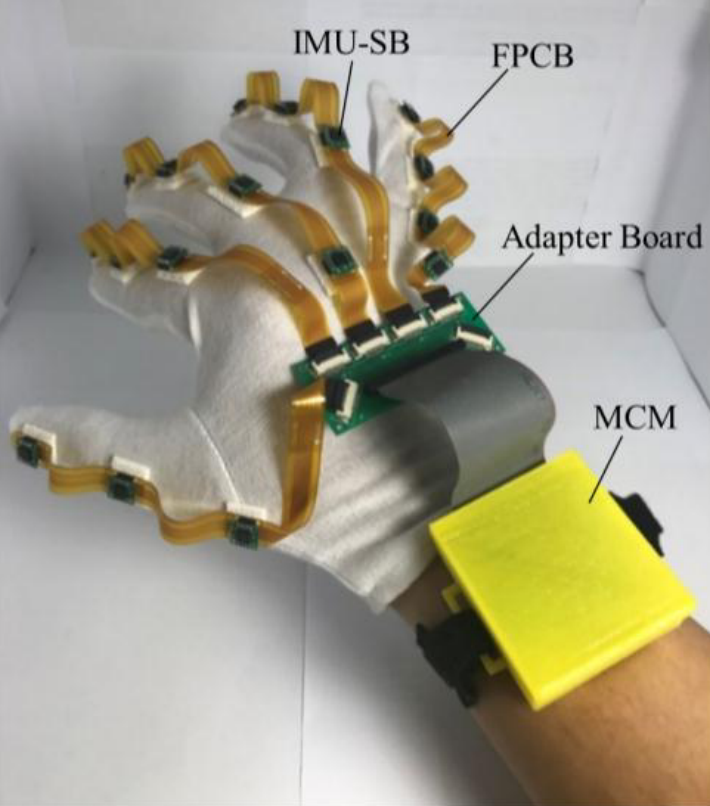
\includegraphics[width=0.6\linewidth]{fig/ch1/data_glove}
  \caption{Data glove\cite{Lin2018}}
  \label{fig:Data glove}
\end{figure}

\subsection*{Motion Capture System}
Motion capture systemはカメラ画像や赤外線距離センサによって,人体の動きをデジタルデータ取得するシステムである.手のモーショントラッキングに特化した,モーションキャプチャシステムにLeap MotionやUbiHand,Digits\cite{Ahmad2006,Kim2012}がある.これらの手法は赤外線カメラにより,手の動きをトラッキングするシステムである.しかし,精度の問題から指の動きといった小さな動きを取得するのは難しい.また,モーションキャプチャシステムを構成する計測機器を常に持ち運んで運用することは難しい.そのため,常に持ち運びができ,精度よく指のトラッキングが行えるシステムが必要である.

\begin{figure}[H]
  \centering
  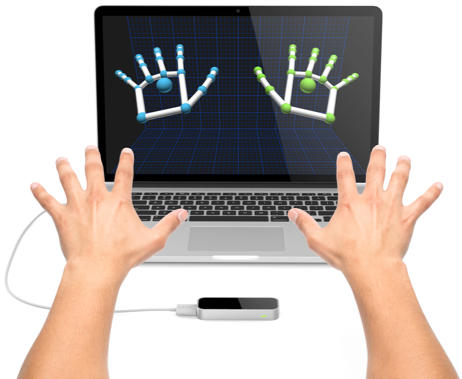
\includegraphics[width=0.6\linewidth]{fig/ch1/mcs}
  \caption{Motion Capture System(Leap Motion)}
  \label{fig:Motion Capture System}
\end{figure}

\subsection*{Manumeter}
Manumeter\cite{Friedman2014}は磁力計と磁石の指輪を用いて手首や指の使用量を測定する手法である.ManumeterをFig.\ref{fig:Manumeter}に示す.手首に取り付けてあるデバイスは磁力計,加速度計とデータ記録のためのストレージ,マイクロコンピュータで構成されている.指の動きを磁石と磁力計間の磁力変化により推定し,指の使用量を測定する.Manumeterは手首の橈屈,尺屈と掌屈,背屈,指の伸展と屈曲を識別する.Manumeterは$R^2 values=0.39–0.61$指の使用量の測定精度が低いという問題点がある.
\begin{figure}[H]
  \centering
  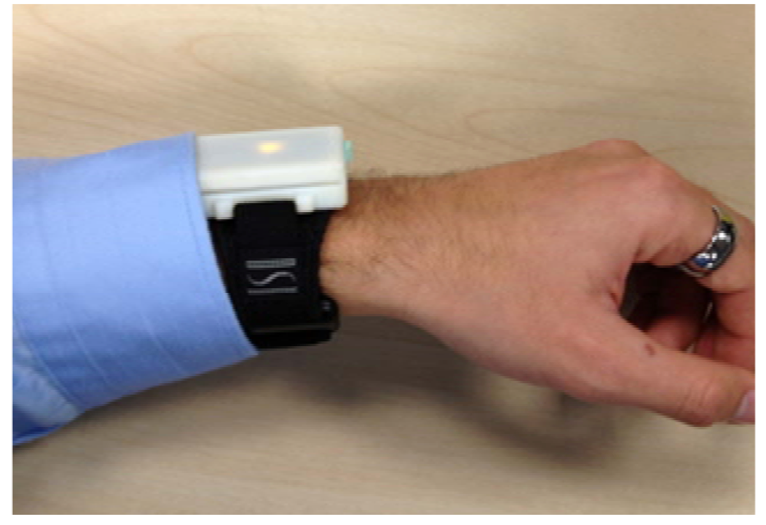
\includegraphics[width=0.6\linewidth]{fig/ch1/manumeter}
  \caption{Manumeter\cite{Friedman2014}}
  \label{fig:Manumeter}
\end{figure}

\subsection*{Behind The Palm}
手の甲の皮膚の皺をパターン認識することによって,指ジェスチャを識別するBehind The Palm\cite{Recognition2017}といった手法が発表されている.ャリブレーションによるユーザーへの負担が大きい,ジェスチャの認識ができるが,精確な手の動作の動きの認識ができないという問題がある.
\begin{figure}[H]
  \centering
  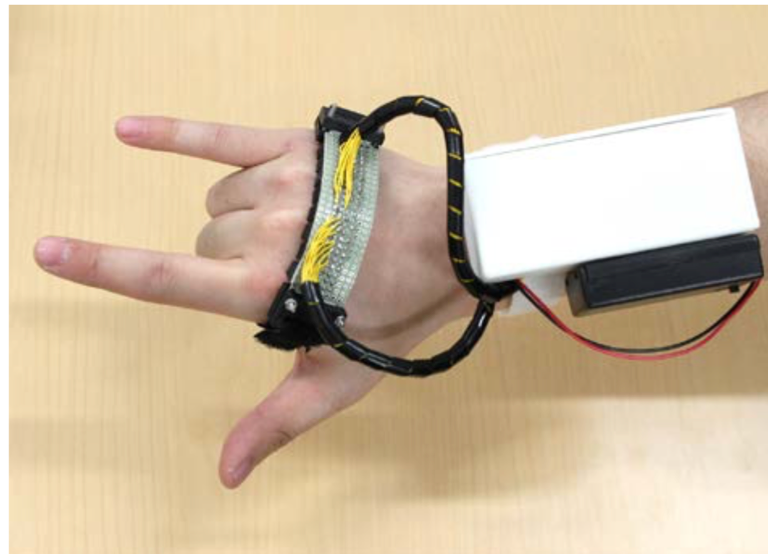
\includegraphics[width=0.6\linewidth]{fig/ch1/btp}
  \caption{Behind The Palm\cite{Recognition2017}}
  \label{fig:Behind The Palm}
\end{figure}

研究レベルではData gloveやGoniometer,Motion capture system\cite{Binh2014,Valtin2017,Chen2003,Ren2011}などが手首や手の使用量を測定するために使用される.しかしながら,これらの手法は指の動きの阻害,空間的な制限といった問題があるため,日常生活における長時間の常時計測には向いていない.

以上の評価手法を表\ref{table:measure}にまとめた.
\begin{table}[H]
  \caption{麻痺肢の評価手法}
  \label{table:measure}
  \centering
  \begin{tabular}{ll}
    \hline
    上肢機能の評価手法 & 強み\\
    \hline \hline 
    診療所や研究所で行われるテスト  & 簡単に短い時間で評価可能  \\
    セルフレポート & 日常生活上での麻痺肢使用を測定できる \\
    Accelerometry  & 定量的に日常生活上での麻痺肢使用を測定可能,患者の動作を阻害しにくい \\
    Data Glove  & 定量的な手指の測定が可能  \\
    Motion Capture System  & 定量的,患者の動きを阻害しない  \\
    Manumeter  & 定量的な手指の測定が可能 \\
    Behind The Palm  & 多くのジェスチャの識別が可能 \\ 
    \hline
  \end{tabular}
\end{table}

\begin{table}[H]
  \caption{麻痺肢の評価手法}
  \label{table:measure}
  \centering
  \begin{tabular}{ll}
    \hline
    上肢機能の評価手法 & 弱み \\
    \hline \hline 
    診療所や研究所で行われるテスト   & 定量的でない,日常生活上の麻痺肢使用を測定できない \\
    セルフレポート & 患者の主観や記憶,認知レベルに評価が左右される,定量的でない\\
    Accelerometry   & ノイズのため,小さな動きや,手指の測定に向かない \\
    Data Glove  &  高価,手を手袋が覆うため,日常生活上の使用に向かない \\
    Motion Capture System   & 高価,空間的な制限がある,高い精度のトラッキングができない \\
    Manumeter  & 磁石を用いるため,複数の指の測定に向かない,精度が低い\\
    Behind The Palm   & キャリブレーションの患者への負担が大きい,ジェスチャのみの測定\\ 
    \hline
  \end{tabular}
\end{table}

\section{リング型デバイス}
\subsection*{ŌURA}




これらの理由から,依然として日常生活下の指の使用量を常時計測する手法は確立していない.本研究では,日常生活下の上肢片麻痺患者の麻痺肢使用,特に指の使用量を測る手法を提案し,手指使用量の常時測定のためのウェアラブルデバイスの開発を目的とする.


\section{本論文の構成}
本論文の構成を以下に記述する.第1章では本研究の背景と既存の研究について紹介する.第2章では,本研究で開発するデバイスの開発方法や,計測されたセンサデータの信号処理について記述する.第3章では,実験方法と結果を記述する.第4章では
実験によって得られた結果に対する考察と,本研究の課題を記述する.
%!TEX root = _thesis.tex
\chapter{手指使用量常時計測の理論と計測ステム構築}

\section{手指使用量の常時計測方法}
既存の手法の問題点を考察すると,手指使用量の常時計測に向いた計測手法は以下の要件を満たす必要がある.

\begin{itemize}
 \item 計測機器が持ち運びやすい
 \item ノイズに対してロバストである
 \item 定量的である
 \item ユーザへの負担が少ない
\end{itemize}

そのため,これらの要件を満たし,手指使用量が計測可能なウェアラブルデバイスの開発を目的とする.計測機器が持ち運びやすいを満たすには,軽量でコンパクトな計測機器が求められる.



\section{指の関節角度計測}
本研究の手指使用量の測定手法は,指の関節角度の変化が,指の使用量を反映するという仮定に基づく.関節角度の変化の推定には,ウェアラブルデバイスに搭載された赤外線距離センサを用いる.本デバイスは指の基節に装着して使用し,赤外線距離センサで,デバイスから中節までの距離を常時計測する.式(1)の関数を用い,測定された距離を指の関節角度に変換し,指の使用量を測る.距離を角度変換する模式図をFig.\ref{fig:principle}に示す.

\begin{figure}[H]
  \centering
  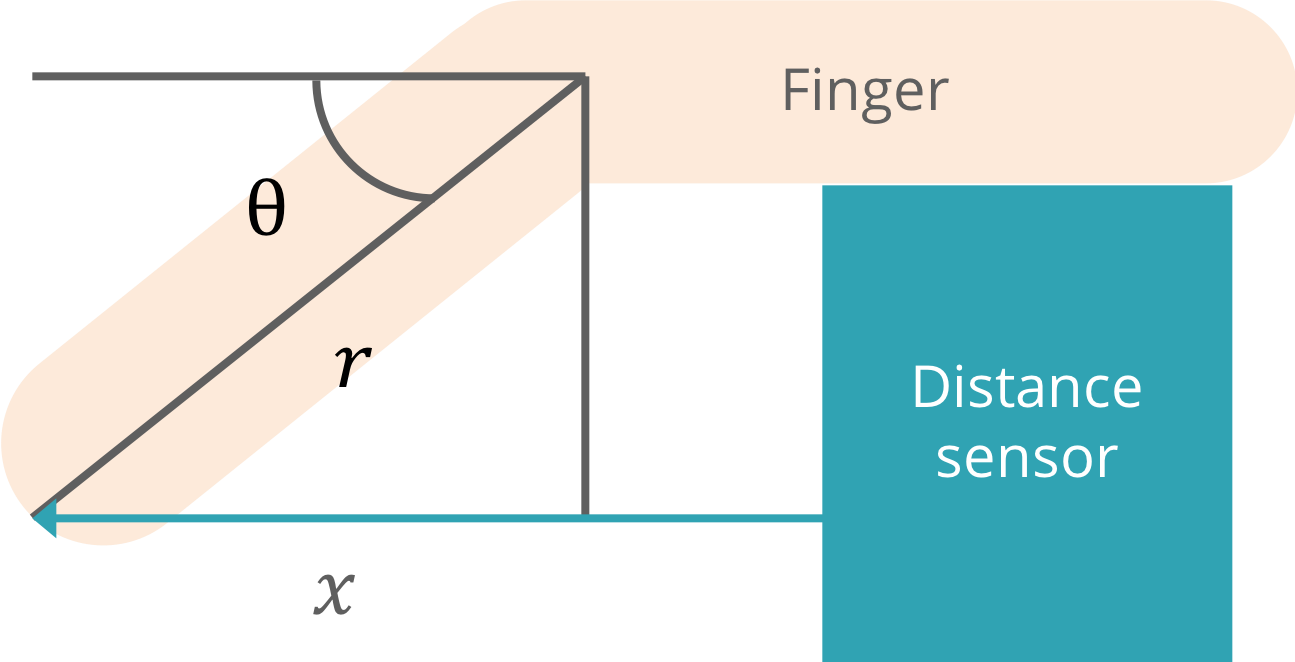
\includegraphics[width=0.8\linewidth]{fig/principle}
  \caption{Measurement principle}
  \label{fig:principle}
\end{figure}

\begin{equation}
\theta = \cos^{-1} \frac{x}{r}
\label{eq:theta}
\end{equation}


ここで,$r$は第二関節から指先までの長さ,$x$は最大屈曲時からの変化距離,$\theta$は最大伸展時からの変化角度である.
$r$はデバイス使用前に物差しやスケール等を用い測定しておく必要がある.$x$は本デバイスの赤外線距離センサによって測定,推定する.この$r,x$の二つのパラメータと式\ref{eq:theta}を用いることで,関節角度$\theta$を導出する.



\section{ウェアラブルデバイスのハードウェア}
本デバイスは加速度計と赤外線距離センサの2つのセンシング部と,センシングされたデータを格納するデータ記録部からなるウェアラブルデバイスである.
本研究で開発したウェアラブルデバイスをFig.\ref{fig:device}に示す.
\begin{figure}[H]
  \centering
  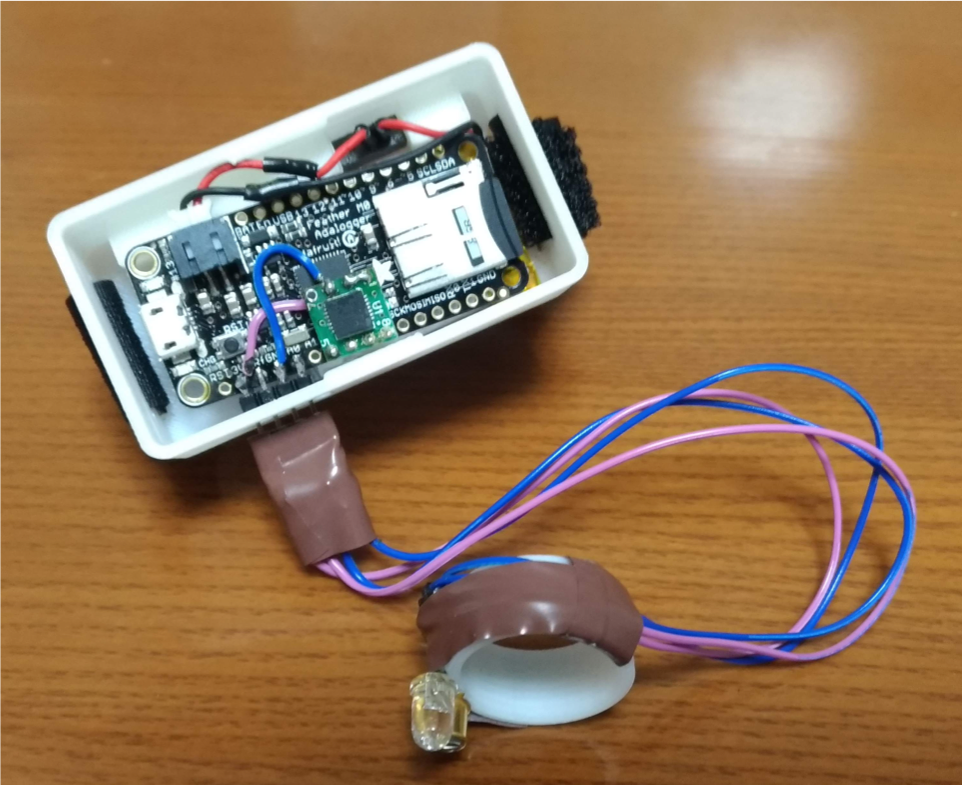
\includegraphics[width=0.8\linewidth]{fig/fal6}
  \caption{Hardware of the wearable device}
  \label{fig:device}
\end{figure}


本デバイスの指輪型の装着部分及び,バッテリーとマイコン基盤を収納するためのケースを3DCAD(Fusion 360)で設計し,3Dプリンタ(Dimension 1200es)で印刷し作成した.


\subsection*{センシング部}
距離計測と加速度計測を行うため,赤外線距離センサと加速度計の二つのセンサを利用した.
\subsubsection*{赤外線距離センサ}
指関節角度の変化をセンシングするため赤外線距離センサを使用した.
赤外線距離センサは発光ダイオード(Osram SFH4550)とフォトトランジスタセンサ(Honeywell SD5410)で構成されている.
赤外線距離センサは発光ダイオードが発光した際に出た光をフォトトランジスタで受光することで,距離を計測するセンサである.
フォトトランジスタの受光量は,ランベルトの反射の性質を有し,光が反射物に反射し受光素子に当たるまでの距離と角度,反射物の反射率により決定される(逆自乗の法則).そのため,センシングキャリブレーションを行った.センシングキャリブレーションに関しては後述する.
外部から入る光によるノイズを抑えるため,発光ダイオードとフォトトランジスタはそれぞれ6$^\circ$と12$^\circ$の狭い視覚野を持つパーツを選定した.手指の関節角度を測定するため,赤外線距離センサを指に取り付ける必要がある.
しかし,直接,テープや手袋などで赤外線距離センサを,ユーザの指に取り付けると,デバイスの装着や取り外しが煩雑になり,
ユーザへの負担が大きくなる問題が生じる.そのため,指輪型のハードウェアへ赤外線距離センサを取り付けた.これにより,ユーザにかかるデバイスの着脱による負荷を低減した.指輪型のハードウェアは3次元コンピュータ支援設計ソフトウェア(Three-dimensional computer-assisted drafting:3DCAD)で設計後,3Dプリンタを用いて作成した.

指輪型ハードウェアの大きさが,ユーザの指の太さと合っていない場合,センサのずれやユーザビリティの低下等の問題が発生する.
ユーザごとに指の太さが異なることが予想されるため,指輪の直径が異なる複数の指輪型のハードウェアを作成した.
AIST\cite{}を参考に,日本人の平均的な食指の直径である,18,19,20,21mmの直径を持つ指輪型ハードウェアを作成した.

\begin{figure}[H]
  \centering
  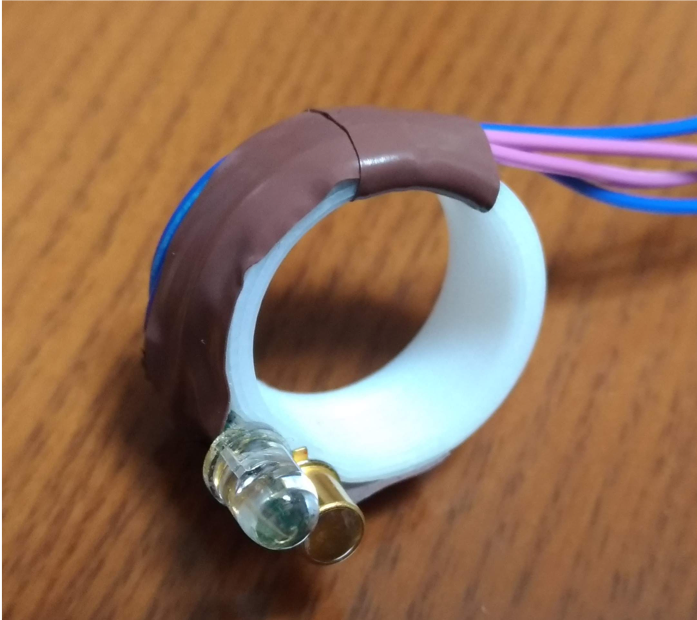
\includegraphics[width=0.8\linewidth]{fig/fal7}
  \caption{Infrared distance sensor consists of LED and Phototransistor}
  \label{fig:distance sensor}
\end{figure}

赤外線距離センサはマイクロコンピュータとワイヤーで接続されており,マイクロコンピュータから給電を行なっている.また,フォトトランジスタがセンシングしたデータをマイクロコンピュータへ出力している.以下のFig.\ref{fig:circuit}に,赤外線距離センサとマイクロコンピュータ(Arduino)の接続を示す.

\begin{figure}[H]
  \centering
  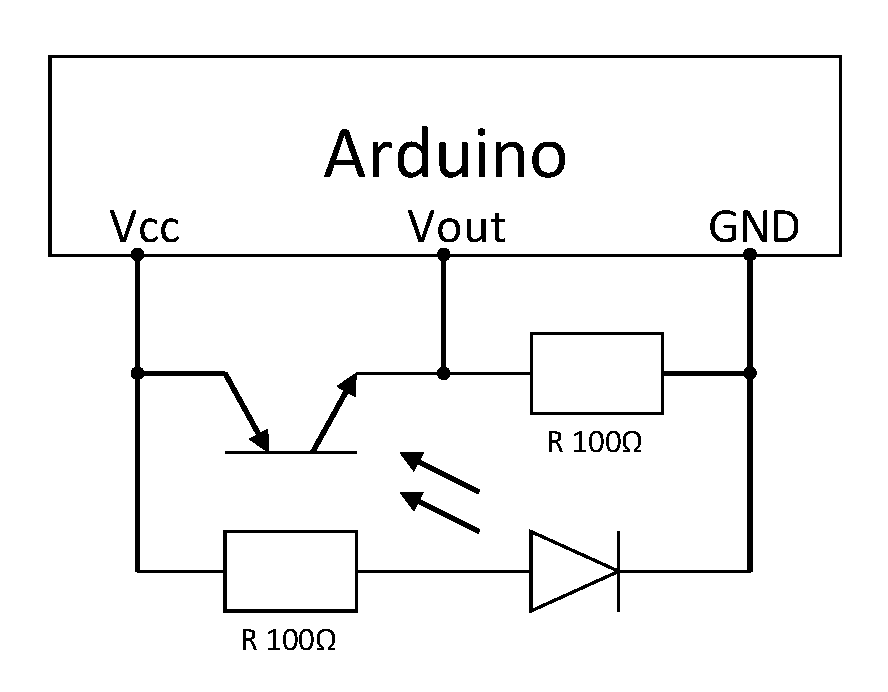
\includegraphics[width=0.5\linewidth]{fig/test}
  \caption{Circuit of the wearable device}
  \label{fig:circuit}
\end{figure}



\subsubsection*{三軸加速度センサ}
さらに,マイコン基盤に三軸加速度センサ(KXR94-2050)を追加した.

\begin{figure}[H]
  \centering
  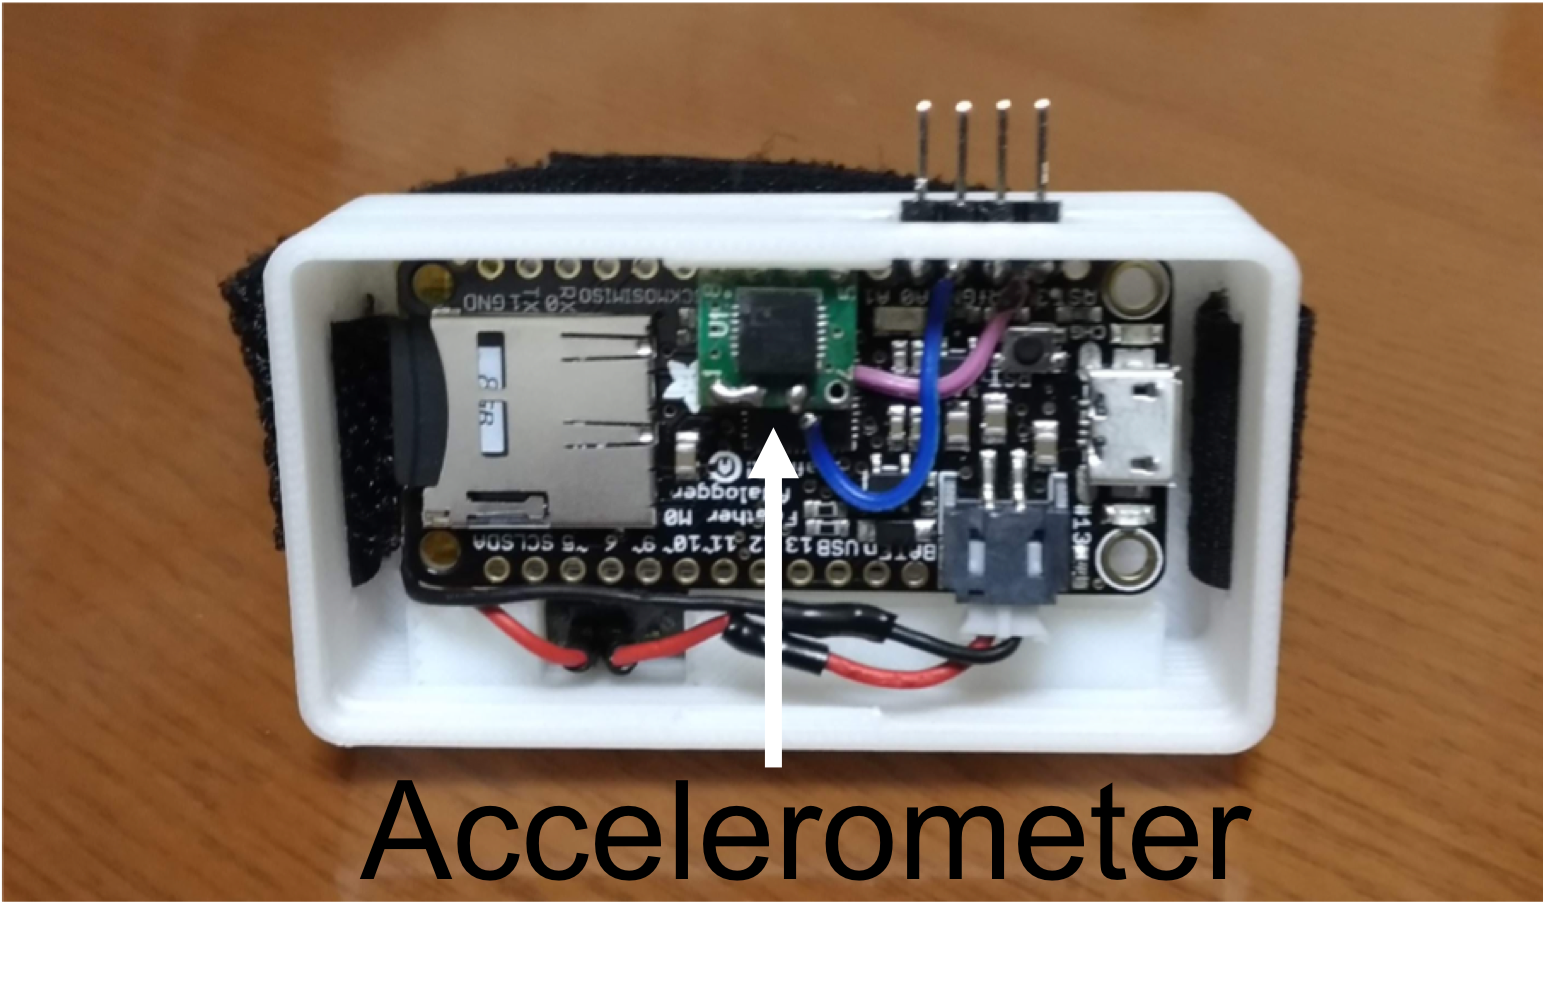
\includegraphics[width=0.5\linewidth]{fig/accelerometer}
  \caption{Accelerometer}
  \label{fig:accelerometer}
\end{figure}

\subsection*{データ記録部}
\subsubsection*{SD card}
データ記録のため,マイコン基盤(Adafruit Faether M0)と32GBのSDcardを使用する.
赤外線距離センサと加速度センサからの信号は,信号の入力時間とともにマイコン基盤に接続されたMicro sdカードへ保存される.コンピュータへUSB2.0 A Male Microケーブルで接続することで,本デバイスのリポバッテリーの充電と,Micro sdカードに記録されたデータの転送が可能である.


\begin{figure}[H]
  \centering
  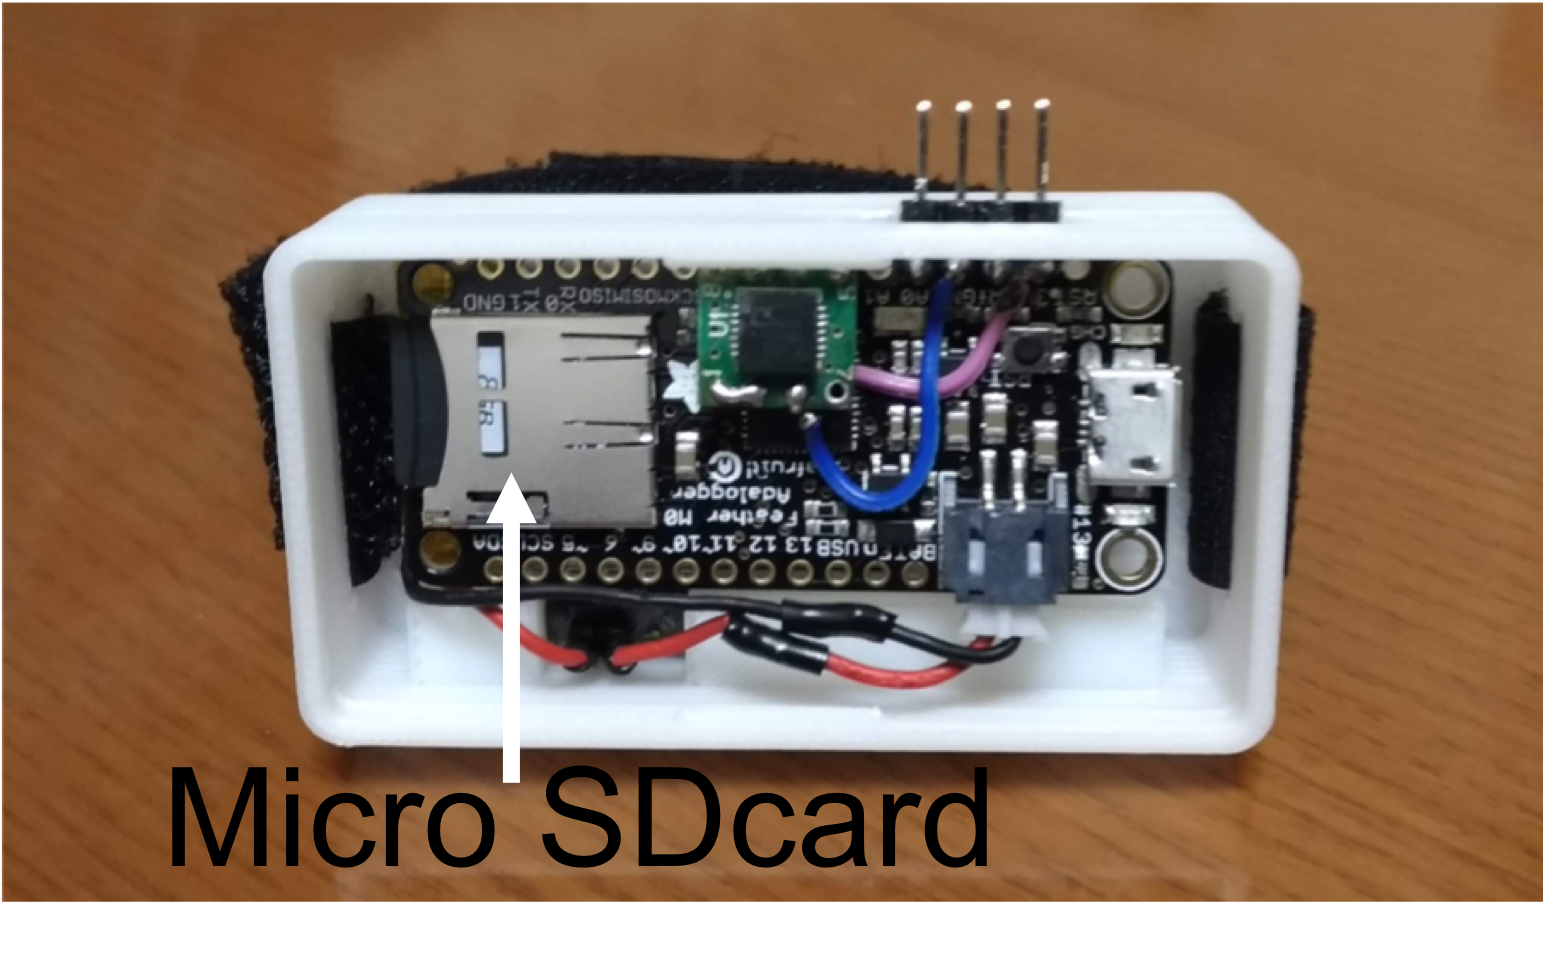
\includegraphics[width=0.5\linewidth]{fig/sdcard}
  \caption{Micro SDcard}
  \label{fig:sd card}
\end{figure}


\subsubsection*{LiPO battery}
デバイスの電源として3.7V,400mAhのリポバッテリーを利用し,これにより24時間以上の連続電源供給が可能である.
\begin{figure}[H]
  \centering
  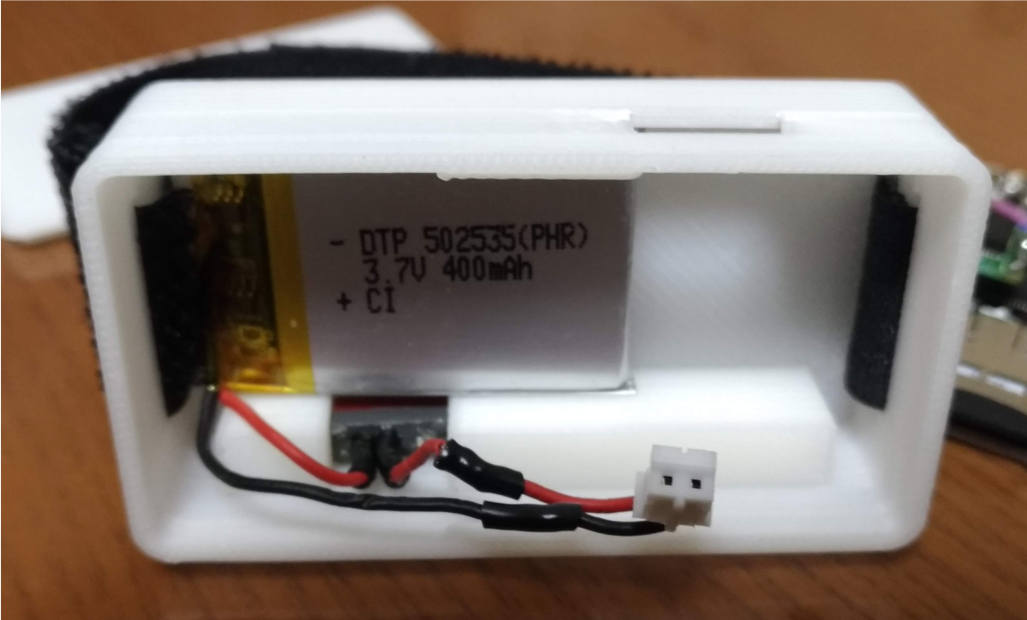
\includegraphics[width=0.5\linewidth]{fig/battery}
  \caption{A LiPO battery}
  \label{fig:battery}
\end{figure}



\subsection*{ウェアラブルデバイスの使用法}
本デバイスに取り付けられたスイッチをオンにすると,赤外線距離センサと加速度センサの記録を開始する.スイッチをオフにするまで連続計測,記録する.データはCSVファイルでSD card内に保存される.本デバイスに記録されたデータは,コンピュータと本デバイスのdeta-logging boardのArduinoをUSBケーブルで直接繋ぐか,Micro SDcardをコンピュータに移すことで,アクセスが可能である.

本デバイスの装着方法をFig\ref{fig:ring}に示す.指輪型のセンシング部は,食指の第二関節に装着し,ストレージ部は手首にマジックテープを使用し取り付ける.



\begin{figure}[H]
  \centering
  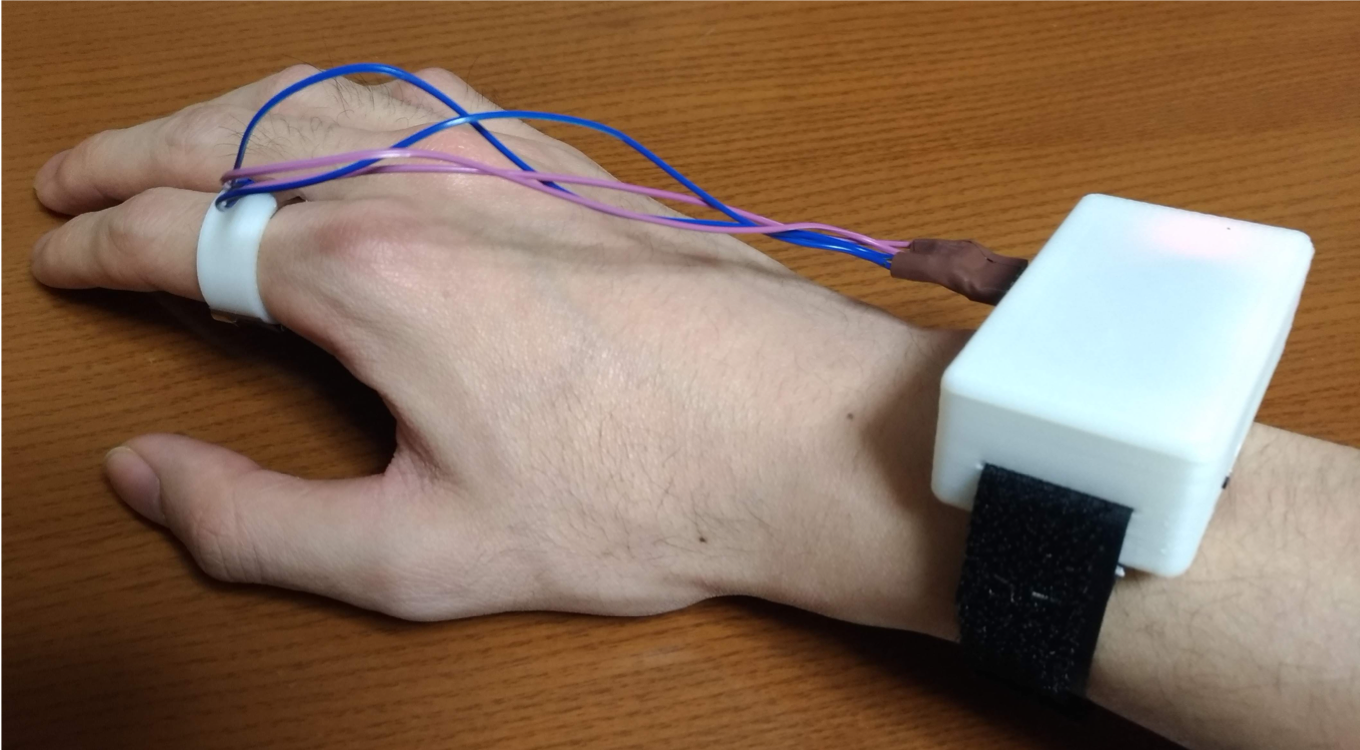
\includegraphics[width=0.8\linewidth]{fig/fal4.png}
  \caption{Ring worn on the index finger and Strage worn on the wrist}
  \label{fig:ring}
\end{figure}


\section{センシングキャリブレーション}
赤外線距離センサは物体に反射し,フォトトランジスタで受光した赤外線の強度を計測することで,距離を推定する.
しかし,同じ距離であっても赤外線が反射する物体によっては,違う
受光量となる場合がありえる.これは物体によって光の反射率が違い,同じ距離で計測したとしても,フォトトランジスタで受け取る受光量が違ってくるためである.つまり,人によって,指の長さや皮膚の色が違うため,同じセンサ値であっても,本来の距離が変わる問題がある.この問題を解決するために,被験者ごとに皮膚の反射率を調べることが望ましいが,本システムは日常生活での使用を目的としており,キャリブレーションがユーザに負荷をかけないことが求められる.
そのため,本システムでは計測される距離と受光量の関係を求め,キャリブレーションが可能な方法を提案する.キャリブレーションには以下の3つのパラメータを用いる.

\begin{itemize}
 \item デバイスを装着する指の長さ
 \item 指伸展時のセンサ情報
 \item 指屈曲時のセンサ情報
\end{itemize}

得られたセンサ情報と指の長さのデータにより,線形近似を行い,ユーザごとのキャリブレーションを行った.




\section{センシング情報の処理方法}
デバイスにより取得できる電圧値は,ノイズを含んでいるため,ノイズの除去を行った.
また,ノイズの除去はバターワイスローパスフィルターにより,10hz以上の周波数を持つシグナルをカットオフすることで行った.赤外線距離センサのセンシングデータから指間接角度を推定する際、いくつかの信号処理を行った.さらに、指の使用量へ変換する処理も行った.それら処理を以下に示す.

\begin{enumerate}
 \item 100Hzのサンプリングレートをもつセンシングデータを10Hzにダウンサンプリングした
 \item  ローパスフィルタにより、ノイズデータを除去した.1次元線形回帰により、センシングデータを,センサから指までの距離へ変換した.
 \item 関節角度が90度,0度のときのセンシングデータを利用し,キャリブレーションを行った
 \item 式\ref{eq:theta}により,距離を角度に変換した
 \item 角度を時間微分し,角度時間の変化角度を導出した
 \item 変化角度の絶対値をとり,タスクごとの指の使用量(タスクの合計変化角度)を導出した.
\end{enumerate}

%!TEX root = _thesis.tex
\chapter{実験手法}

\section{指の長さ計測}
本デバイスのキャリブレーションには,ユーザの指の長さデータが必要である.そのため,ユーザの食指の第二関節から指先までの長さをメジャーを用い,計測した.実験の被験者の食指の第二関節から指先までの長さのデータを以下に示す.また,第二指長の計測結果を以下に示す.被験者は8名が男性,2名が女性である.

\begin{table}[H]
  \caption{Length between fingertip and proximal interphslangeal joint with index finger(n=10)}
  \label{table:finger_distance}
  \centering
  \begin{tabular}{ccccc}
    \hline
    Subjects & Length(cm)& Length(cm) & Sex & Dominant Hand\\
    \hline \hline 
    A  & 2.71 & 0.993 & Female & Left\\
    B  & 2.62 & 0.995 & Male & Right\\
    C  & 6.61 & 0.985 & Male & Right\\
    D  & 5.01 & 0.994 & Male & Right\\
    E  & 2.33 & 0.995 & Male & Right\\ 
    F  & 2.87 & 0.995 & Male & Right\\
    G  & 1.57 & 0.998 & Male & Right\\
    H  & 2.87 & 0.992 & Male & Right\\
    I  & 3.04 & 0.986 & Female & Right\\
    J  & 2.41 & 0.994 & Male & Right\\
    \hline
  \end{tabular}
\end{table}

実験の被験者の食指の第二関節から指先までの長さの平均と標準偏差は,

また,第二指長の平均と標準偏差は


\section{ジェスチャ識別精度の評価}
予備実験として健常者を対象に,本システムのジェスチャの認識精度を調査した.この実験の際は,LED(Osram SFH4550)とフォトトランジスタセンサ(Honeywell SD5410)の代わりに,赤外線距離センサ(Pololu QTR-1A)を2つ使用し,Fig.\ref{fig:sensor}の位置に取り付けた.

\begin{figure}[H]
  \centering
  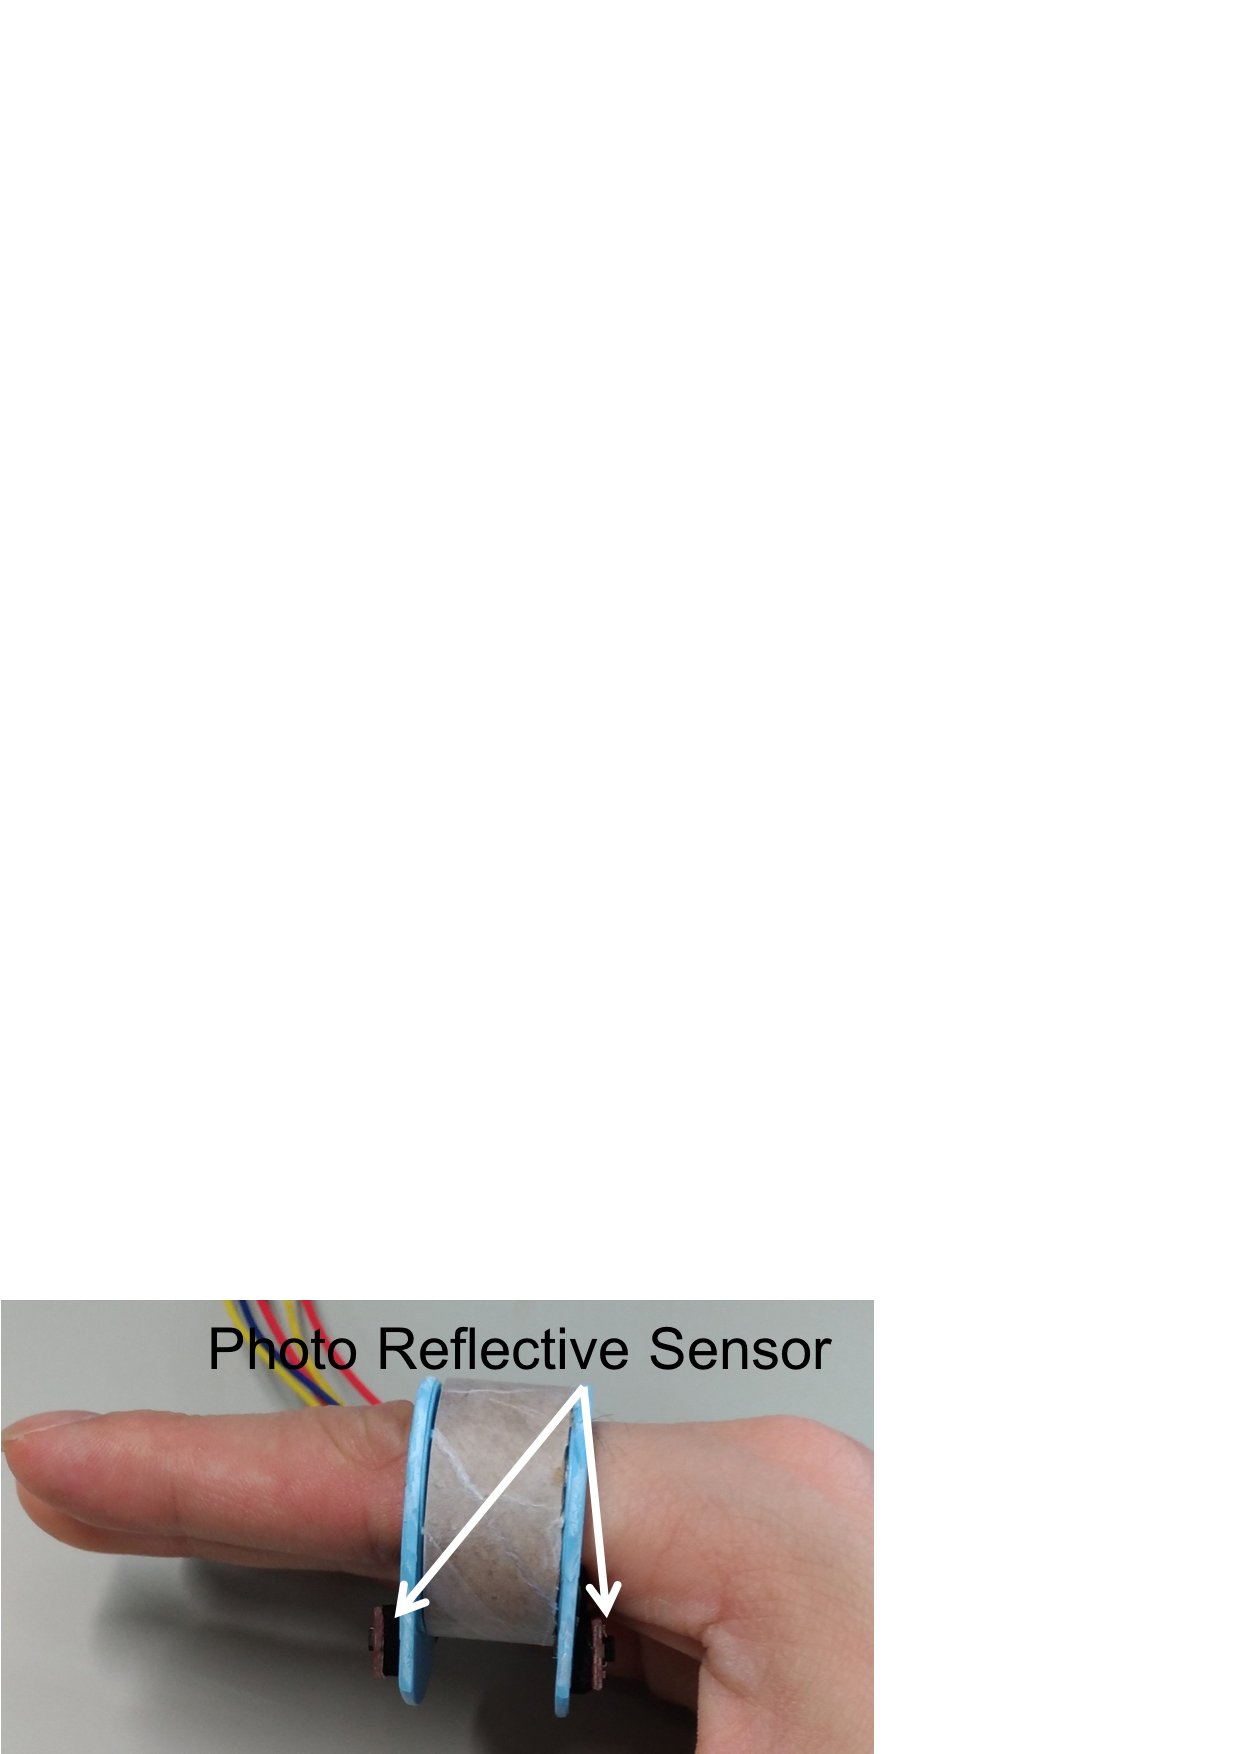
\includegraphics[width=0.6\linewidth]{fig/sensor}
  \caption{Mounting position of sensor}
  \label{fig:sensor}
\end{figure}

ジェスチャの種類をFig.\ref{fig:gesture}に示す.手指を閉じた状態(Fig.\ref{fig:gesture}の1),示指と母指で輪を作った状態(Fig.\ref{fig:gesture}の2),手指を開いた状態(Fig.\ref{fig:gesture}の3),計三つのジェスチャを指示し被験者に行ってもらった.これらのジェスチャは\cite{Lin2015}を元にした.被験者は椅子に座った状態で,本デバイスを装着した手でジェスチャを行った.被験者は一つのジェスチャを5秒間保持する.ジェスチャ時のセンサーデータを収集した.ジェスチャを5秒間保持している時の,センサ値の標準偏差は推定角度に変換すると被験者平均でSD=$\pm0.12度$であり,ごく小さいものだった.5秒間のセンサーデータを時間で平均したセンサ値をジェスチャ識別のために利用した.
また,センサデータは各ジェスチャにつき60回記録し,五人の被験者センサデータを収集した.センシングの際のサンプルレートは100\ Hzとした.
合計で一人につき180データ(60データ$\times$3ジェスチャ)を収集した.

\begin{figure}[H]
  \centering
  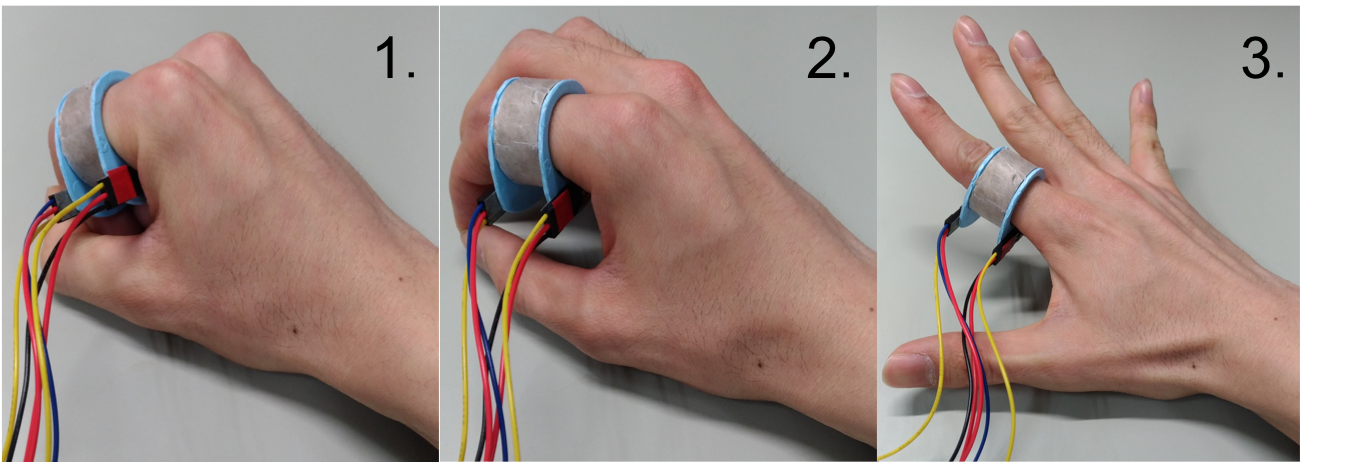
\includegraphics[width=0.8\linewidth]{fig/gesture}
  \caption{Prepared hand-gesture set}
  \label{fig:gesture}
\end{figure}

三つのジェスチャを識別するため,一対一分類法,線形Support Vector Machineを用いた.五人すべて,900データ(180データ$\times$五人)をジェスチャごとにラベル分けし,ジェスチャ識別に利用した.これらのデータの内,各ラベルに対し,データの80\%をトレーニングデータ,20\%をテストデータとし,5-fold cross validationを行なった.


\section{関節角度推定精度の評価}
健常者十人を対象に本デバイスの関節角度の推定精度の評価を行なった.被験者の指の関節を0$\sim$90°まで15°刻みで固定し,その時の関節角度の推定精度を評価した.指関節角度の固定には以下のFig\ref{fig:kotei}に示す器具を使用する.この器具は3DCAD(Fusion 360)で設計し,3Dプリンタ(Dimension 1200es)で印刷し作成した.この器具をFig.\ref{fig:kotei}(b)に示すとおり,食指の第二関節にあて関節角度を固定する.Fig.\ref{fig:kotei}(b)では$45^\circ$に固定されている.


\begin{figure}[H]
\begin{center}
\begin{tabular}{cc}
\subfigure[Fixture]{
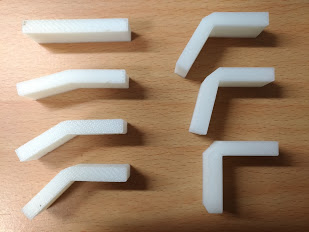
\includegraphics[scale=0.5]{fig/kotei}
} &
\subfigure[Fixture used to fix a finger]{
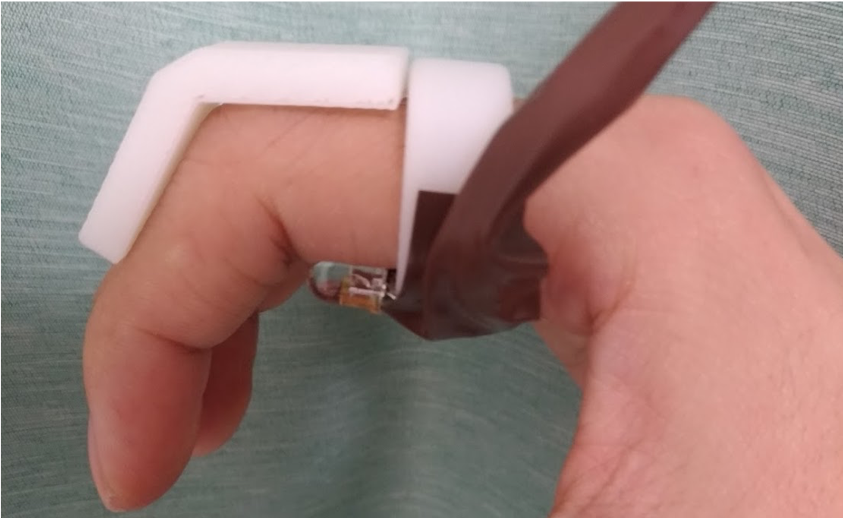
\includegraphics[scale=0.5]{fig/kotei1}
} \\
\end{tabular}
\end{center}
\caption{Finger fixing}
\label{fig:kotei}
\end{figure}

指を固定した状態で,赤外線距離センサのセンシングを行い,その時の関節角度と,推定された関節角度を比較した.デバイスを装着後,器具を装着し,指の角度を固定する.その状態で,センサデータの計測を3秒間行った.さらに,各角度につき10回計測を行った.被験者一人につき,70回計測を行った.被験者数は十人,センサのサンプルレートは100Hzとした.精度評価の際,推定角度と正解角度の絶対誤差の平均値Mean Absolute Error(MAE)と相関係数Rを評価指標とした.
\begin{equation}
MAE = \frac{1}{n} \sum^n_{k=1} |Res_i|
\label{eq:mae}
\end{equation}

\begin{equation}
Res_i = Pred_i - True_i
\label{eq:res}
\end{equation}

$Pred_iとTrue_i$はそれぞれ,計測$i$回目の時の推定角度と正解角度を示している.推定角度は,赤外線距離センサからの信号に処理を加え,Fig.\ref{fig:principle}に示す関係より推定した角度である.正解角度は,センシング時に指関節にあてているFig.\ref{fig:kotei}に示した,0$\sim$90$^\circ$の固定器具の角度である.
また,$Res_i$は$i$回目の計測時の正解角度と推定角度の誤差を示す.


\section{Acceleromertyとの日常生活,リハビリ動作評価の比較}
既存手法のAcceleromertyと本手法の比較を行った.
accelerometryでは,感知できなかった指の使用動作を検知できるか
本デバイスに加速度センサを搭載し,実験を行なった.


本手法により,日常生活動作の評価が可能かを調査した.調査の方法を以下に示す.
六つのタスクをそれぞれ5分間,合計30分間,以下の順番で八人の被験者が行った.
被験者は左利きが一人,右利きが七人であり,二人が女性,六人が男性であった.
また全ての被験者は健常者であった.実験を行う際,Fig.\ref{fig:ring}に示すように,三軸加速度計(データ記録部)を被験者の両手首,赤外線距離センサを両手の食指に装着し同時計測した.

本実験で被験者に指示したタスクを以下に示す.
\begin{table}[H]
  \begin{tabular}{cc}
    \hline 
    Tasks&   Details\\
        \hline \hline
箸を使い食事&
被験者は利き手に箸を持ち,三つの皿に分けられた食品を口に運び食す.\\

布巾でテーブルを拭く&
被験者は利き手に布巾を持ち,70cm四方のテーブルを拭く.\\

タイピング&
被験者は両手を用い,タイピングゲームを行う.\\

ライティング&
被験者は利き手にボールペンを持ち,文字の書き取りを行う.\\

布巾を畳む&
被験者は両手を用い,布巾を四つ折りに畳む,広げるを繰り返す.\\

Hole peg testを行う&
被験者は利き手で十本のペグをホールに入れ,全てのペグをホールから抜き出すを繰り返す.\\

    \hline
  \end{tabular}
\end{table}

これらのタスクは生活日常動作五つと,リハビリテーション動作のBox and block testからなり,\cite{Taub2011,Mathiowetz1985}を参考にした.
タスクの説明をもっと詳しく書く.

%!TEX root = _thesis.tex
\chapter{考察と課題}

\section{結論}
リハビリテーション介入の効果を定量的に測定する手法として,手指使用量の常時計測のためのウェアラブルデバイスの開発を行った.本デバイスは赤外線距離センサを用いて指の第二関節角度を推定する指輪型のデバイスである.結果より,本手法により関節角度を推定でき,手指使用量を計測可能であることが示唆された.


\begin{itemize}
 \item 
 \item 
 \item 
\end{itemize}


\section{課題}
日常生活動作を一日中測定することは難しい.
・水に濡れる
・デバイスが有線であるため,邪魔になる可能性
エンジニアリングで解消できる.

\chapter{考察と課題}

\section{結論}
リハビリテーション介入の効果を定量的に測定する手法として,手指使用量の常時計測のためのウェアラブルデバイスの開発を行った.本デバイスは赤外線距離センサを用いて指の第二関節角度を推定する指輪型のデバイスである.結果より,本手法により関節角度を推定でき,手指使用量を計測可能であることが示唆された.


%%!TEX root = _thesis.tex
\chapter*{謝辞}
本研究の一部は,JSPS KAKENHI (JP26120005,JP16H03219) の支援による.ここに謝意を表す.




%\bibliography{ref}

\bibliographystyle{jplain}
\bibliography{library}
[65]河内まき子,2012,AIST日本人の手の寸法データ,https://unit.aist.go.jp/hiri/dhrg/ja/dhdb/hand/index.html

\newpage
\printindex
\end{document}